\documentclass[man, fleqn, noextraspace,floatsintext]{apa6}
\usepackage{lmodern}
\usepackage{amssymb,amsmath}
\usepackage{ifxetex,ifluatex}
\usepackage{fixltx2e} % provides \textsubscript
\ifnum 0\ifxetex 1\fi\ifluatex 1\fi=0 % if pdftex
  \usepackage[T1]{fontenc}
  \usepackage[utf8]{inputenc}
\else % if luatex or xelatex
  \ifxetex
    \usepackage{mathspec}
  \else
    \usepackage{fontspec}
  \fi
  \defaultfontfeatures{Ligatures=TeX,Scale=MatchLowercase}
\fi
% use upquote if available, for straight quotes in verbatim environments
\IfFileExists{upquote.sty}{\usepackage{upquote}}{}
% use microtype if available
\IfFileExists{microtype.sty}{%
\usepackage{microtype}
\UseMicrotypeSet[protrusion]{basicmath} % disable protrusion for tt fonts
}{}
\usepackage{hyperref}
\hypersetup{unicode=true,
            pdftitle={Trends in Major League Sports in the U.S. from 2000-2015},
            pdfauthor={Woocheol Kim~\& Jessica Canfield},
            pdfkeywords={sports, NBA, NHL, NFL, MLB, NCAAF},
            pdfborder={0 0 0},
            breaklinks=true}
\urlstyle{same}  % don't use monospace font for urls
\usepackage{graphicx,grffile}
\makeatletter
\def\maxwidth{\ifdim\Gin@nat@width>\linewidth\linewidth\else\Gin@nat@width\fi}
\def\maxheight{\ifdim\Gin@nat@height>\textheight\textheight\else\Gin@nat@height\fi}
\makeatother
% Scale images if necessary, so that they will not overflow the page
% margins by default, and it is still possible to overwrite the defaults
% using explicit options in \includegraphics[width, height, ...]{}
\setkeys{Gin}{width=\maxwidth,height=\maxheight,keepaspectratio}
\IfFileExists{parskip.sty}{%
\usepackage{parskip}
}{% else
\setlength{\parindent}{0pt}
\setlength{\parskip}{6pt plus 2pt minus 1pt}
}
\setlength{\emergencystretch}{3em}  % prevent overfull lines
\providecommand{\tightlist}{%
  \setlength{\itemsep}{0pt}\setlength{\parskip}{0pt}}
\setcounter{secnumdepth}{0}
% Redefines (sub)paragraphs to behave more like sections
\ifx\paragraph\undefined\else
\let\oldparagraph\paragraph
\renewcommand{\paragraph}[1]{\oldparagraph{#1}\mbox{}}
\fi
\ifx\subparagraph\undefined\else
\let\oldsubparagraph\subparagraph
\renewcommand{\subparagraph}[1]{\oldsubparagraph{#1}\mbox{}}
\fi

%%% Use protect on footnotes to avoid problems with footnotes in titles
\let\rmarkdownfootnote\footnote%
\def\footnote{\protect\rmarkdownfootnote}


  \title{Trends in Major League Sports in the U.S. from 2000-2015}
    \author{Woocheol Kim\textsuperscript{1}~\& Jessica Canfield\textsuperscript{1}}
    \date{}
  
\shorttitle{Exploring Trends in Major League Sports }
\affiliation{
\vspace{0.5cm}
\textsuperscript{1} University of Oregon}
\keywords{sports, NBA, NHL, NFL, MLB, NCAAF}
\usepackage{csquotes}
\usepackage{upgreek}
\captionsetup{font=singlespacing,justification=justified}

\usepackage{longtable}
\usepackage{lscape}
\usepackage{multirow}
\usepackage{tabularx}
\usepackage[flushleft]{threeparttable}
\usepackage{threeparttablex}

\newenvironment{lltable}{\begin{landscape}\begin{center}\begin{ThreePartTable}}{\end{ThreePartTable}\end{center}\end{landscape}}

\makeatletter
\newcommand\LastLTentrywidth{1em}
\newlength\longtablewidth
\setlength{\longtablewidth}{1in}
\newcommand{\getlongtablewidth}{\begingroup \ifcsname LT@\roman{LT@tables}\endcsname \global\longtablewidth=0pt \renewcommand{\LT@entry}[2]{\global\advance\longtablewidth by ##2\relax\gdef\LastLTentrywidth{##2}}\@nameuse{LT@\roman{LT@tables}} \fi \endgroup}


\usepackage{lineno}

\linenumbers

\authornote{Jessica Canfield \& Woocheol Kim are both
Marketing PhD students at the University of Oregon.

Correspondence concerning this article should be addressed to Woocheol
Kim, 1208 University St, Eugene, OR 97403. E-mail:
\href{mailto:wkim4@uoregon.edu}{\nolinkurl{wkim4@uoregon.edu}}}

\abstract{
Marketing research has frequently used the context of sports to explore
one facet of consumption. Additionally, the data within the sports realm
is well-documented and detailed across time which allows for analyses to
be tracked across time and different locations. While the current
analysis is mainly exploratory in nature the goal of this project is to
familiarize ourselves with this dataset prior to using it in future
marketing studies. In this project specifically we look at how the 2008
financial crisis impacts ticket price for professional sports teams.
However, in the future we plan to use this data in conjunction with
other datasets that have unique time and location identifiers to look
more specifically at how consumers engage with sports in reaction to
other events occuring simultaneously, whether that be financial crises,
political uncertainty, or natural disasters.


}

\begin{document}
\maketitle

\section{Introduction}\label{introduction}

Humphreys (2010) explores the impact of the global financial crisis on
sport in North America. He finds that while attendance and franchise
values declined slightly, and a few teams experienced notable financial
problems, the nature of sports as a consumer product in addition to
institutional factors associated with the sports industry have, so far,
insulted professional sports from significant negative shocks as the
result of economic uncertainty. Coates and Humphreys (2007) investigate
the demand for attendance at professional sporting events using a data
set that includes ticket prices and a price index reflecting prices for
ancillary goods associated with attendance. Both mathematical modeling
and empirical methodology are used in their research (see Coates \&
Humphreys, 2007).

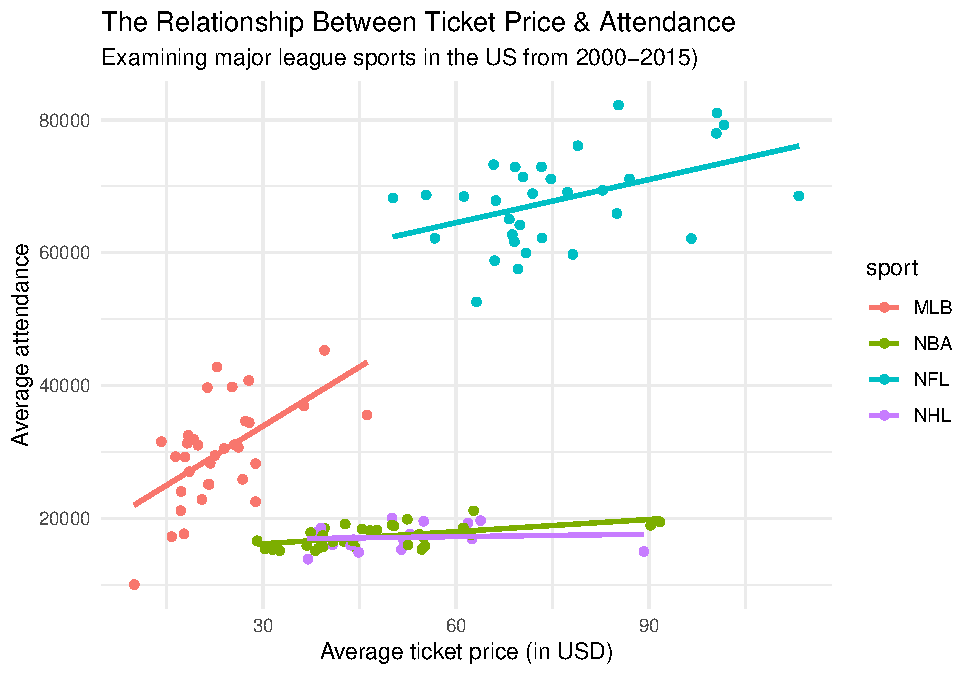
\includegraphics{Final_Project_files/figure-latex/plots-1.pdf}
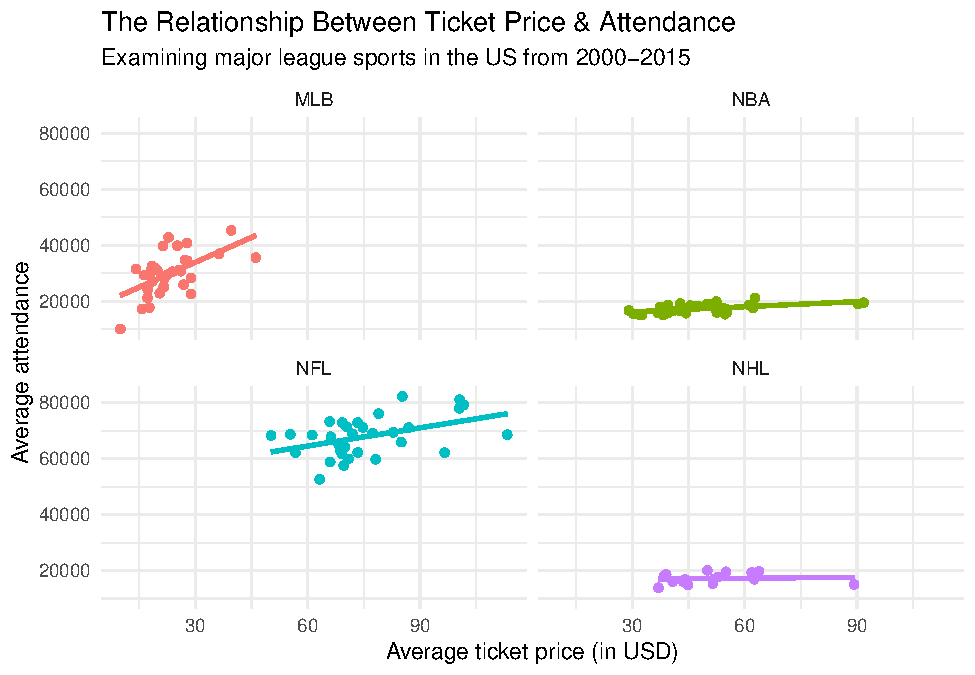
\includegraphics{Final_Project_files/figure-latex/plots-2.pdf}
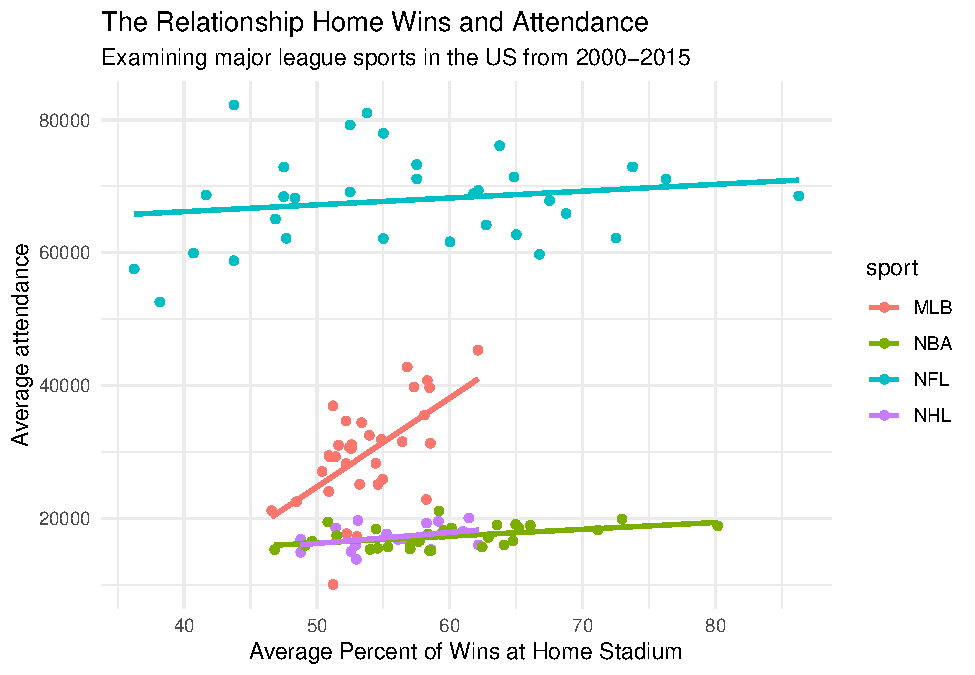
\includegraphics{Final_Project_files/figure-latex/plots-3.pdf}
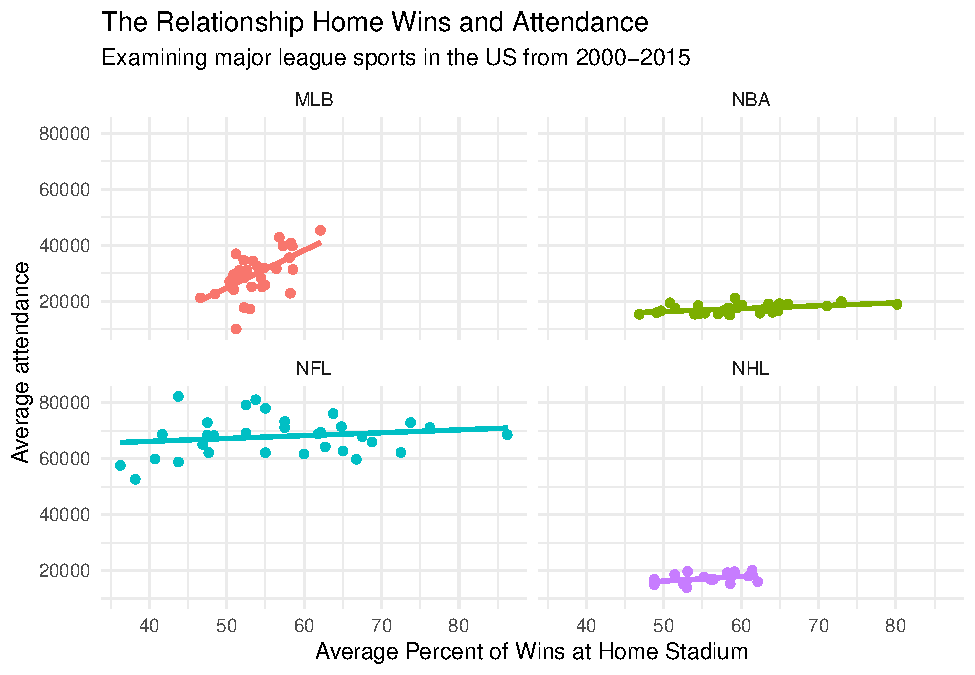
\includegraphics{Final_Project_files/figure-latex/plots-4.pdf}

\begin{figure}
\centering
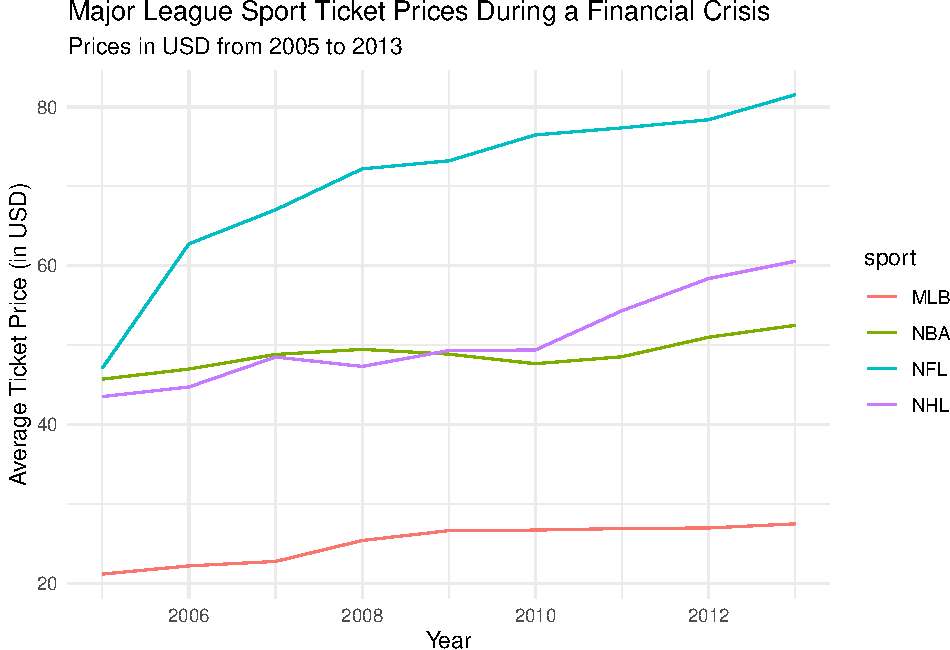
\includegraphics{Final_Project_files/figure-latex/sports_crisis-1.pdf}
\caption{}
\end{figure}

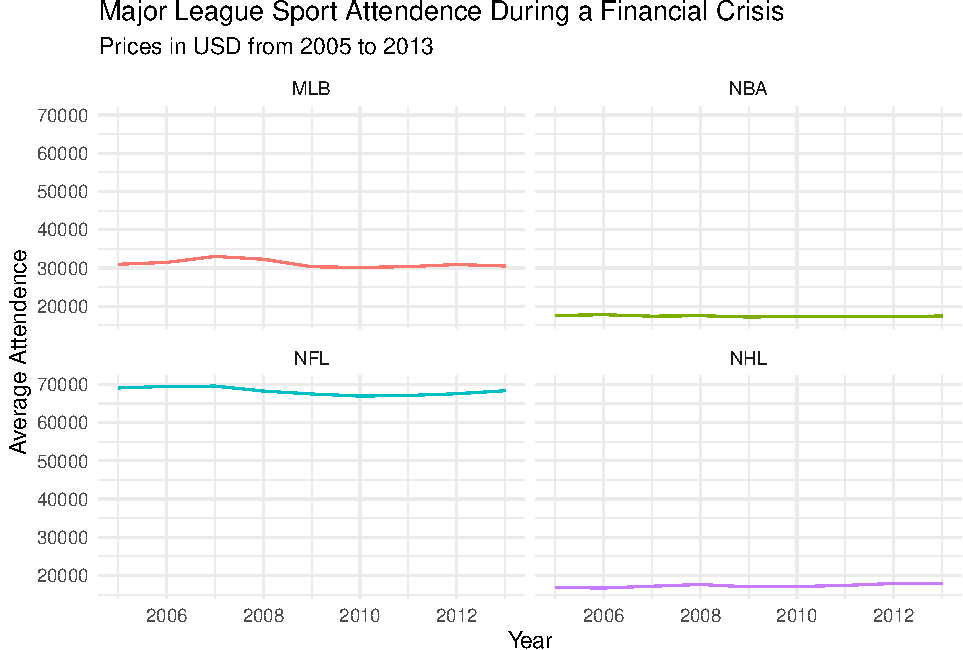
\includegraphics{Final_Project_files/figure-latex/unnamed-chunk-1-1.pdf}
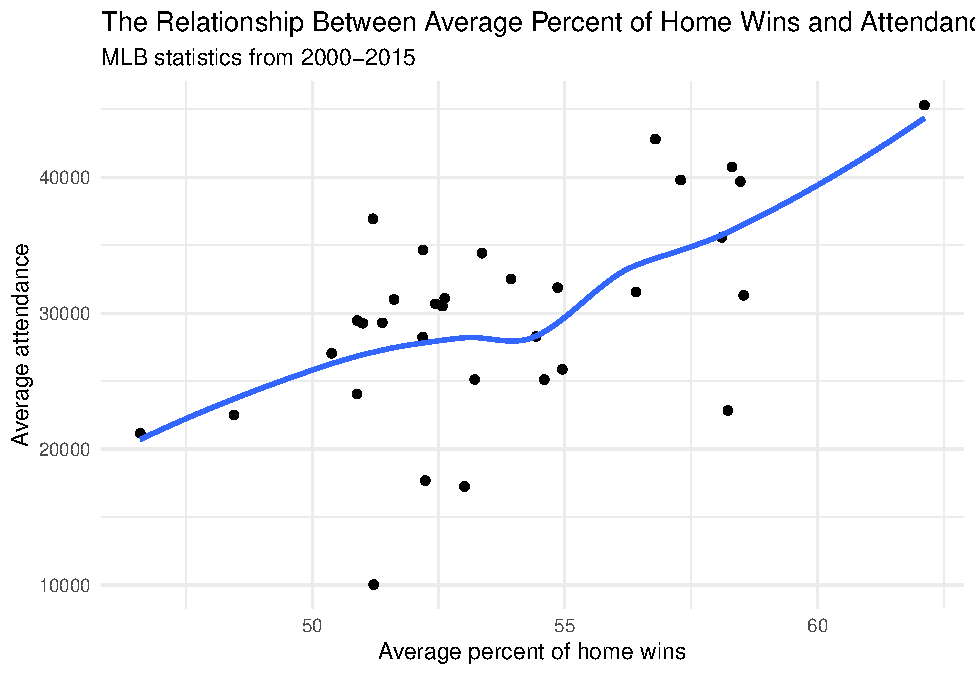
\includegraphics{Final_Project_files/figure-latex/unnamed-chunk-1-2.pdf}

\subsection{Average Home Attendance, Average Home Ticket Price and
Average Home Win pct by Sports
(2000-2015)}\label{average-home-attendance-average-home-ticket-price-and-average-home-win-pct-by-sports-2000-2015}

\begin{tabular}{l|r|r|r}
\hline
sport & attendance\_mean & ticketprice\_mean & homewinpct\_mean\\
\hline
MLB & 30420.90 & 23.51 & 53.88\\
\hline
NBA & 17335.68 & 49.04 & 59.70\\
\hline
NFL & 68039.56 & 75.29 & 56.86\\
\hline
NHL & 17342.74 & 51.76 & 55.94\\
\hline
\end{tabular}

Average revenue per homegame for Major league Baseball (MLB) teams
spanning from 2007 and 2009 is \$794,445.22 while the one for three
years after \textbf{financial crisis} is \$818,114.18. Major League
Baseball seems that it was not affected by recesesion in terms of
\emph{revenue} and it actually made more than before the crisis.
However, to understand how the recession impacted MLB in greater detail
we would need to account for other variables.

\subsection{Average Home Game Revenue before and after economic
recession}\label{average-home-game-revenue-before-and-after-economic-recession}

Average revenue per homegame of MLB spanning from 2007 and 2009 is
\$794,445.22 while the revenue 3 years after the \textbf{financial
crisis} is \$818,114.18. Major League Baseball seems that it was not
affected by depression in terms of \emph{revenue} and it actually made
more than before the crisis.

\section{Methods}\label{methods}

The sports dataset was collected by marketing professor Conor Henderson.
It covers four major league sports (NBA, MLB, NFL, NHL) as well as NCAA
college football (NCAAF). For each sport, the data spans from 2000
through 2015 and is currently in the process of being updated through
present. The data was originally compiled from a number of reputable
sports-focused sources including Rodney Fort's Sports League Database as
well as ESPN. In the final dataset that combines all the sports we have
1398 observations across 15 years and 10 different variables. The 10
variables we selected were: sport, team, year, stadium capacity, total
attendance, average attendance, number of games, ticket price (in USD),
and the number of home wins.

\subsection{Data analysis}\label{data-analysis}

We used R (Version 3.6.1; R Core Team, 2019) and the R-packages
\emph{dplyr} (Version 0.8.3; Wickham, François, Henry, \& Müller, 2019),
\emph{forcats} (Version 0.4.0; Wickham, 2019a), \emph{ggplot2} (Version
3.2.1; Wickham, 2016), \emph{here} (Version 0.1; Müller, 2017),
\emph{janitor} (Version 1.2.0; Firke, 2019), \emph{kableExtra} (Version
1.1.0; Zhu, 2019), \emph{knitr} (Version 1.25; Xie, 2015), \emph{lme4}
(Bates, Mächler, Bolker, \& Walker, 2015), \emph{Matrix} (Version
1.2.17; Bates \& Maechler, 2019), \emph{papaja} (Version 0.1.0.9842;
Aust \& Barth, 2018), \emph{purrr} (Version 0.3.3; Henry \& Wickham,
2019), \emph{readr} (Version 1.3.1; Wickham, Hester, \& Francois, 2018),
\emph{rio} (Version 0.5.16; C.-h. Chan, Chan, Leeper, \& Becker, 2018),
\emph{stringr} (Version 1.4.0; Wickham, 2019b), \emph{tibble} (Version
2.1.3; Müller \& Wickham, 2019), \emph{tidyr} (Version 1.0.0; Wickham \&
Henry, 2019), and \emph{tidyverse} (Version 1.2.1; Wickham, 2017) for
all our analyses.

\section{Results}\label{results}

In all four leagues, it turns out that average ticket price and average
rate of home wins is positively associated with average home attendance
even though NFL fans seem they are not as sensitive to wins as are the
fans in the three other major league sports. This provides empirical
evidence for a finding that is relativley intuitive in the sense that as
teams win more, demand for tickets likely increases which would drive
prices up. Ultimatley, people enjoy watching their home team win and as
a result, are willing to pay more when their team is doing well in a
given season. However, this is likely correlated with the outcomes of
previous seasons as well. In all four leagues, it turns out that average
ticket price and average home win rate have a positive relationship with
average home attendance even though NFL fans seem to be not as sensitive
to win as other three leagues' fans are. In addition, the 2008 financial
crisis did not result in crisis in the US professional sports leagues.
While some of the leagues experienced slight decrease in home
attendance, all four leagues got through economic downturn as if there
was nothing happened. Actually, their home game average revenue went up
after financial crisis. We assume this counterintuitive outcome is
attributed to the facts that sports were kind of immuned to the crisis
for some reason or even during recession people are willing to spend
money for watching games.

\section{Discussion}\label{discussion}

Sports continue to play an important role in the United States. In an
time when individuals are becoming increasingly isolated
{[}Chalmers2012differences;Shachar2011brands{]}, sports games provide a
form of entertainment from that can be bring people together, whether
that be through watching the game at the sadium or field or on
television. While the motivation to watch sports differs for
individuals, the widespread appeal of watching teams compete provides a
context for marketers to understand sponshorship, group marketing
strategies, and targeted advertising. The current exploratory study
provides inital insight into how major league attendance varries over
time both in regard to attedance as well as ticket prices. Through the
analysis, it is clear that each of the major league sports operates very
differently from eachother inregard to the variables of interest
isolated for the purposes of this research. As this dataset it used
going forward, it will be important to identify more clearly the
differences between each of the sports to understand if they can indeed
be collapsed into an overarching category of \enquote{major league
sports attendance} across all four major league sports (MLB, NBA, NFL,
NHL). Another aspect that was not taken into account in the current
research is team-specific factors including how long the team has been
in a city as well as how many time a team has moved.

\newpage

\section{References}\label{references}

\begingroup
\setlength{\parindent}{-0.5in} \setlength{\leftskip}{0.5in}

\hypertarget{refs}{}
\hypertarget{ref-R-papaja}{}
Aust, F., \& Barth, M. (2018). \emph{papaja: Create APA manuscripts with
R Markdown}. Retrieved from \url{https://github.com/crsh/papaja}

\hypertarget{ref-R-Matrix}{}
Bates, D., \& Maechler, M. (2019). \emph{Matrix: Sparse and dense matrix
classes and methods}. Retrieved from
\url{https://CRAN.R-project.org/package=Matrix}

\hypertarget{ref-R-lme4}{}
Bates, D., Mächler, M., Bolker, B., \& Walker, S. (2015). Fitting linear
mixed-effects models using lme4. \emph{Journal of Statistical Software},
\emph{67}(1), 1--48. \url{https://doi.org/10.18637/jss.v067.i01}

\hypertarget{ref-R-rio}{}
Chan, C.-h., Chan, G. C., Leeper, T. J., \& Becker, J. (2018).
\emph{Rio: A swiss-army knife for data file i/o}.

\hypertarget{ref-coates_humphreys_2007}{}
Coates, D., \& Humphreys, B. R. (2007). Ticket prices, concessions and
attendance at professional sporting events. \emph{International Journal
of Sport Finance}, \emph{2}(3), 161.

\hypertarget{ref-R-janitor}{}
Firke, S. (2019). \emph{Janitor: Simple tools for examining and cleaning
dirty data}. Retrieved from
\url{https://CRAN.R-project.org/package=janitor}

\hypertarget{ref-R-purrr}{}
Henry, L., \& Wickham, H. (2019). \emph{Purrr: Functional programming
tools}. Retrieved from \url{https://CRAN.R-project.org/package=purrr}

\hypertarget{ref-humphreys_2010}{}
Humphreys, B. R. (2010). The impact of the global financial crisis on
sport in north america. In \emph{Optimal strategies in sports economics
and management} (pp. 39--57). Springer.

\hypertarget{ref-R-here}{}
Müller, K. (2017). \emph{Here: A simpler way to find your files}.
Retrieved from \url{https://CRAN.R-project.org/package=here}

\hypertarget{ref-R-tibble}{}
Müller, K., \& Wickham, H. (2019). \emph{Tibble: Simple data frames}.
Retrieved from \url{https://CRAN.R-project.org/package=tibble}

\hypertarget{ref-R-base}{}
R Core Team. (2019). \emph{R: A language and environment for statistical
computing}. Vienna, Austria: R Foundation for Statistical Computing.
Retrieved from \url{https://www.R-project.org/}

\hypertarget{ref-R-ggplot2}{}
Wickham, H. (2016). \emph{Ggplot2: Elegant graphics for data analysis}.
Springer-Verlag New York. Retrieved from
\url{https://ggplot2.tidyverse.org}

\hypertarget{ref-R-tidyverse}{}
Wickham, H. (2017). \emph{Tidyverse: Easily install and load the
'tidyverse'}. Retrieved from
\url{https://CRAN.R-project.org/package=tidyverse}

\hypertarget{ref-R-forcats}{}
Wickham, H. (2019a). \emph{Forcats: Tools for working with categorical
variables (factors)}. Retrieved from
\url{https://CRAN.R-project.org/package=forcats}

\hypertarget{ref-R-stringr}{}
Wickham, H. (2019b). \emph{Stringr: Simple, consistent wrappers for
common string operations}. Retrieved from
\url{https://CRAN.R-project.org/package=stringr}

\hypertarget{ref-R-tidyr}{}
Wickham, H., \& Henry, L. (2019). \emph{Tidyr: Tidy messy data}.
Retrieved from \url{https://CRAN.R-project.org/package=tidyr}

\hypertarget{ref-R-dplyr}{}
Wickham, H., François, R., Henry, L., \& Müller, K. (2019). \emph{Dplyr:
A grammar of data manipulation}. Retrieved from
\url{https://CRAN.R-project.org/package=dplyr}

\hypertarget{ref-R-readr}{}
Wickham, H., Hester, J., \& Francois, R. (2018). \emph{Readr: Read
rectangular text data}. Retrieved from
\url{https://CRAN.R-project.org/package=readr}

\hypertarget{ref-R-knitr}{}
Xie, Y. (2015). \emph{Dynamic documents with R and knitr} (2nd ed.).
Boca Raton, Florida: Chapman; Hall/CRC. Retrieved from
\url{https://yihui.name/knitr/}

\hypertarget{ref-R-kableExtra}{}
Zhu, H. (2019). \emph{KableExtra: Construct complex table with 'kable'
and pipe syntax}. Retrieved from
\url{https://CRAN.R-project.org/package=kableExtra}

\endgroup


\end{document}
